\documentclass[12pt,a4paper]{article} 

\usepackage[spanish]{babel} 
\usepackage[utf8]{inputenc}
\usepackage[numbers,sort&compress]{natbib} 
\usepackage{graphicx} 
\usepackage{amsfonts}
\usepackage[left=2cm,right=2cm,top=2cm,bottom=2cm]{geometry}
\usepackage{listings}
\usepackage[usenames,dvipsnames]{color}
\usepackage{float}
\usepackage{natbib}

\author{Cynthia Ivanna Cruz Quiñones\\
Matricula: 1854499\\ Grupo: 002}
\title{Matemáticas Computacionales\\ Práctica 3\\
Métodos de Bisección}
\date{A 26 de Marzo del 2021}


\begin{document}
\maketitle
\newpage

\section{Introdcción}
En esta práctica 3 se implementa un método de Análisis Numérico para determinar los ceros de una función. En general, encontrar los ceros de una función en un número finito pasos casi nunca es posible. Para ello se utilizan métodos de aproximación. Estos métodos son iterativos iniciando con una aproximacón $x_{0}$ o un intervalo $[a, b]$, calculamos aproximaciones sucesivas $x_{1}, x_{2},..., x_{n}$ y se escoge $x_{n}$ como aproximación del cero de la función cuando se cumpla un criterio de paro. \citep{repositorio}


\section{Método de Bisección}
Este es uno de los métodos más sencillos y de fácil intuición, para resolver ecuaciones en una variable. Se basa en el Teorema de los Valores Intermedios, el cual establece que toda función continua $f$ en un intervalo cerrado [$a,b$] ($f \epsilon C[a,b]$) toma todos los valores que se hallan entre $f(a)$ y $f(b)$. Esto es, que todo valor entre $f(a)$ y $f(b)$ es la imagen de al menos un valor en el intervalo [$a,b$]. 

Observe la siguiente figura \ref{fig:MB}

\begin{figure}[h]
\centering
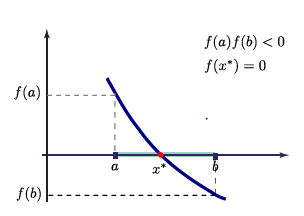
\includegraphics[scale=1.0]{MB}
\caption{Representación grafica}
\label{fig:MB}
\end{figure}

El método consiste en lo siguiente: Supongamos que en el intervalo [$a,b$] hay un cero de $f$. Calculamos el punto medio $m=\frac{a+b}{2}$ del intervalo [$a,b$] A continuación calculamos $f(m)$. En caso de que $f(m)$ sea igual a cero, ya hemos encontrado la solución buscada. En caso de que no lo sea, verificamos si $f(m)$ tiene signo opuesto al de $f(a)$. Se redefine el intervalo [$a,b$] como [$a,m$] o [$m,b$] según se haya determinado en cuál de estos intervalos ocurre un cambio de signo. A este nuevo intervalo se le aplica el mismo procedimiento y así, sucesivamente, iremos encerrando la solución en un intervalo cada vez más pequeño, hasta alcanzar la precisión deseada. 

La siguiente representación gráfica \ref{fig:MB_01} se muestra el procedimiento descrito. 

\newpage

\begin{figure}[h]
\centering
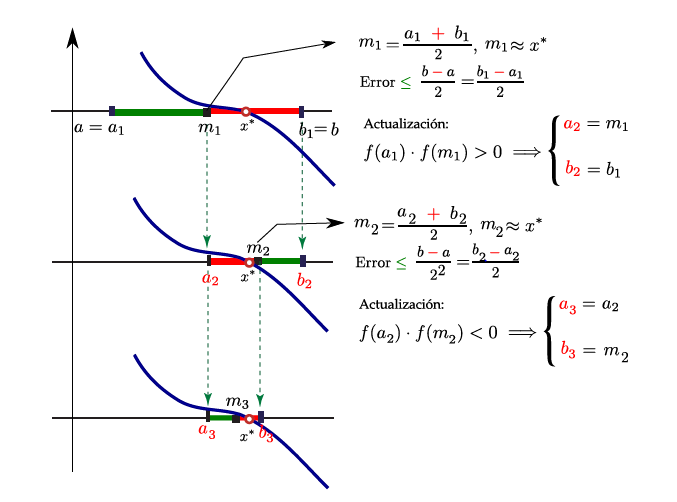
\includegraphics[scale=0.8]{MB_01}
\caption{El procedimiento construye tres sucesiones $a_{n}$, $b_{n}$, $m_{n}$}
\label{fig:MB_01}
\end{figure}

Para $k = 1, 2, ..., m_{k}=\frac{b_{k}+ a_{k}}{2}$ y  

\begin{equation}
[a_{k},b_{k}] = \left\lbrace
\begin{array}{ll}
\textup{} [m_{k-1}, b_{k-1}] &si f(a_{k-1})f(m_{k-1})>0 \\
\textup{} [a_{k-1}, m_{k-1}] &si f(a_{k-1})f(m_{k-1})<0
\end{array}
\right.
\end{equation}


\subsection{Estimación del error}
El error exacto en el k-ésimo paso en $|m_{k} - x^{*}|$.
Geométricamente se puede ver esto que esto es menos que la mitad del intervalo $|a_{k} - b_{k}|$ , esto quiere decir que


\begin{equation}
    |m_{k} - x^{*}| \leq \frac{b_{k}-a_{k}}{2}= \frac{b-a}{2^{k}}
\end{equation}

Esto se muestra en la siguiente figura \ref{fig:MB_02}

\begin{figure}[ht]
\centering
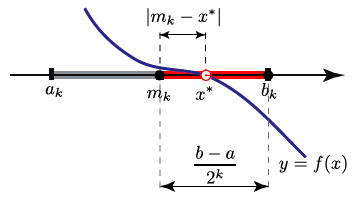
\includegraphics[scale=1]{MB_02}
\caption{Estimación del error en bisección.}
\label{fig:MB_02}
\end{figure}


\section{Tarea}

\textbf{1.- Para $x^3=0$ con bisección en $[-0.2,0.1]$} 

La tolerancia dada para esta funcion fue de $0.000001$ por lo que la función necesito de $18$ iteraciones para encontrar los ceros dentro de el intervalo dado. [tabla \ref{Funcion1}] y su representación gráfica en la figura \ref{fig:Funcion1}

\begin{figure}[h]
\centering
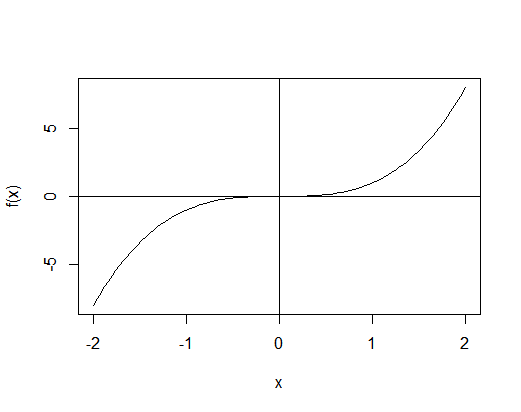
\includegraphics[scale=0.6]{Funcion1}
\caption{Función $x^3=0$ con bisección $[-0.2,0.1]$ y de curva de $(-2,2)$}
\label{fig:Funcion1}
\end{figure}

\begin{table}[ht]
\centering
\begin{tabular}{|c|c|c|c|}
\hline
a          & b         & m          & Error est. \\ \hline
-0.0500000 & 0.1000000 & -0.0500000 & 0.0750000  \\ \hline
-0.0500000 & 0.0250000 & 0.0250000  & 0.0375000  \\ \hline
-0.0125000 & 0.0250000 & -0.0125000 & 0.0187500  \\ \hline
-0.0125000 & 0.0062500 & 0.0062500  & 0.0093750  \\ \hline
-0.0031250 & 0.0062500 & -0.0031250 & 0.0046875  \\ \hline
-0.0031250 & 0.0015625 & 0.0015625  & 0.0023437  \\ \hline
-0.0007812 & 0.0015625 & -0.0007812 & 0.0011719  \\ \hline
-0.0007812 & 0.0003906 & 0.0003906  & 0.0005859  \\ \hline
-0.0001953 & 0.0003906 & -0.0001953 & 0.0002930  \\ \hline
-0.0001953 & 0.0000977 & 0.0000977  & 0.0001465  \\ \hline
-0.0000488 & 0.0000977 & -0.0000488 & 0.0000732  \\ \hline
-0.0000488 & 0.0000244 & 0.0000244  & 0.0000366  \\ \hline
-0.0000122 & 0.0000244 & -0.0000122 & 0.0000183  \\ \hline
-0.0000122 & 0.0000061 & 0.0000061  & 0.0000092  \\ \hline
-0.0000031 & 0.0000061 & -0.0000031 & 0.0000046  \\ \hline
-0.0000031 & 0.0000015 & 0.0000015  & 0.0000023  \\ \hline
-0.0000008 & 0.0000015 & -0.0000008 & 0.0000011  \\ \hline
-0.0000008 & 0.0000004 & 0.0000004  & 0.0000006  \\ \hline
\end{tabular}
\caption{Tabla de iteración}
\label{Funcion1}
\end{table}

Cero de $f$ en $[-0.2 , 0.1]$ es approx:  $3.814697e-07$ con $error \Leftarrow 5.722046e-07$

\newpage
\textbf{2.- Para $x^5 - 100x^4 + 3995x^3 - 79700x^2 + 794004x - 3160075$ con bisección en $[17,22.2]$}

Esta cuenta con 22 iteraciónes, de las cuales solo se muestran las primeras 5 y ultimas dos generadas por la consola en la tabla \ref{Funcion2} al igual que la gráfica generada representada en la figura \ref{fig:Funcion2}, de la cual se tiene una tolerancia de $0.000001$ y dentro del intervalo dado con curva de $(-200,200)$
 
\begin{figure}[h]
\centering
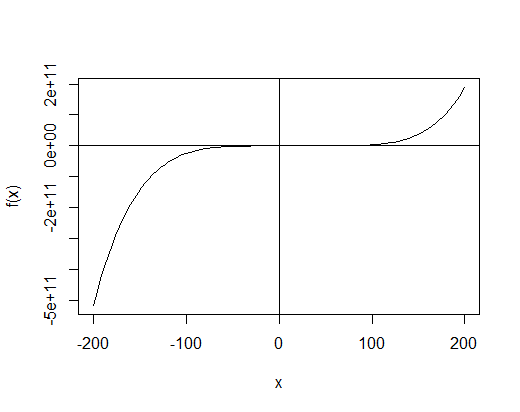
\includegraphics[scale=0.6]{Funcion2}
\caption{Función $x^5 - 100x^4 + 3995x^3 - 79700x^2 + 794004x - 3160075$ con bisección en $[17,22.2]$}
\label{fig:Funcion2}
\end{figure}

\begin{table}[ht]
\centering
\begin{tabular}{|c|c|c|c|}
\hline
a          & b          & m          & Error est. \\ \hline
17.0000000 & 19.6000000 & 19.6000000 & 1.3000000  \\ \hline
17.0000000 & 18.3000000 & 18.3000000 & 0.6500000  \\ \hline
17.6500000 & 18.3000000 & 17.6500000 & 0.3250000  \\ \hline
17.6500000 & 17.9750000 & 17.9750000 & 0.1625000  \\ \hline
....       & ....       & ....       & ....       \\ \hline
17.8463633 & 17.8463657 & 17.8463633 & 0.0000012  \\ \hline
17.8463645 & 17.8463657 & 17.8463645 & 0.0000006  \\ \hline
\end{tabular}
\caption{Tabla de iteración de la función 2}
\label{Funcion2}
\end{table}

Cero de $f$ en $[17 , 22.2]$ es approx:  $17.84636$ con $error \Longleftarrow 6.198883e-07$




\textbf{3.- Para $x^3-2x-5=0$}

En esta función se generaron 21 iteraciones con una tolerancia de $0.000001$ y bisección en $[2.094,5]$, de las cuales se presentan las primeras 5 y las ultimas dos en la tabla \ref{Figura3} y su representacion gráfica en la figura \ref{fig:Funcion3}; depende de la tolerancia para el numero de iteraciones que se generan.
Se toma el 2.094 ya que la raiz de la función $x^3-2x-5=0$ es 2.094564. 

\begin{figure}[ht]
\centering
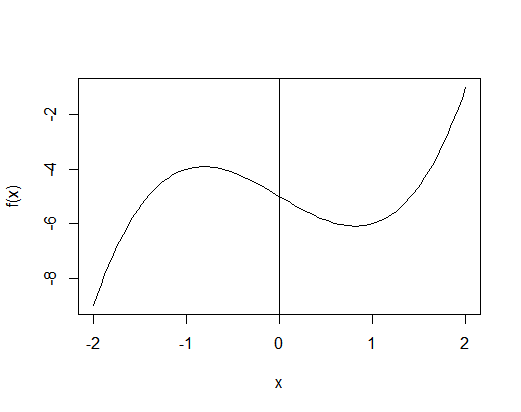
\includegraphics[scale=0.6]{Funcion3}
\caption{Función $x^3-2x-5=0$}
\label{fig:Funcion3}
\end{figure}

\begin{table}[ht]
\centering
\begin{tabular}{|c|c|c|c|}
\hline
a         & b         & m         & Error est. \\ \hline
2.0000000 & 3.5000000 & 3.5000000 & 0.7500000  \\ \hline
2.0000000 & 2.7500000 & 2.7500000 & 0.3750000  \\ \hline
2.0000000 & 2.3750000 & 2.3750000 & 0.1875000  \\ \hline
2.0000000 & 2.1875000 & 2.1875000 & 0.0937500  \\ \hline
....      & ....      & ....      & ....       \\ \hline
2.0945511 & 2.0945539 & 2.0945539 & 0.0000014  \\ \hline
2.0945511 & 2.0945525 & 2.0945525 & 0.0000007  \\ \hline
\end{tabular}
\caption{Tabla de iteración para la funcón $x^3-2x-5=0$}
\label{Figura3}
\end{table}

Cero de $f$ en $[2.094 , 5]$ es approx:  $2.09455$ con $error <=\Leftarrow 6.928444e-07$


\bibliography{biblio}
\bibliographystyle{plainnat}



\end{document}